%%
%% Author: dariochinelli
%% 2021-03-25
%%

\section{Meccanica Statistica}
La meccanica statistica si utilizza in contesti in cui il sistema fisico è costituito da un elevato numero di elementi.
Se ad esempio consideriamo una mole di un gas stiamo considerando un sistema con \SI{6.02e23}{} particelle (corrispondente al numero di Avogadro $N_A$), risulterà quindi impossibile utilizzare un approccio in cui studiare il comportamento e l'evoluzione delle singole particelle.
Si usa allora un approccio statistico, mediando posizioni e velocità, questo metodo è utilizzato ad esempio per sistemi termodinamici.

\textit{Particella} viene utilizzato in senso ampio per indicare ogni unità ben definita che compone il sistema, potrà essere un atomo, una molecola, un elettrone e così via.

Considero un sistema di $N$ particelle
\begin{equation}
n_1,n_2,n_3, ...
\end{equation}
e considero che ogniuna abbia a disposizione diversi livelli di energia 
\begin{equation}
E_1,E_2,E_3, ...
\end{equation}
in cui si può trovare, tali stati potranno essere discreti e ben distanziati oppure tanto vicini da formare quasi un continuo.
Se assumiamo che tali stati siano discreti e che ogni particella $n_i$ si trovi in uno stato di energia $E_i$, allora il numero totale di particelle è dato da
\begin{equation}
N = n_1 + n_2 + n_3 + ... = \sum_s n_s
\end{equation}
che risulta essere una costante e l'energia totale del sistema è
\begin{equation}
U_{tot} = n_1 E_1 + n_2 E_2 + ... = \sum_s n_s E_s
\end{equation}
che, considerando un sistema isolato, risulta anch'essa una costante.

Esistono più distribuzioni possibili per le particelle fra i vari livelli energetici, che sono dette \textit{partizioni}, e per ogni stato macroscopico del sistema (definito da N, U, dal tipo di particella, ecc...) esiste una partizione più probabile delle altre.
Quando il sistema raggiunge la partizione più probabile allora il sistema è all'\textit{equilibrio statistico} e tenderà a rimanerci fintanto che non subentrerà un agente esterno.

Per studiare un sistema statistico dobbiamo trovare la partizione più probabile che corrisponde a trovare la legge di distribuzione, da cui potremo dedurre le proprietà macroscopiche del sistema che saranno le proprietà medie del sistema complessivo.

Come si ottengono le leggi di distribuzione? Vedremo ora tre casi:
la statistica classica, nel caso in cui le particelle siano distinguibili, e le statistiche quantistiche per indistinguibili, quindi bosoni e fermioni.


\subsection{Statistica classica di Maxwell Boltzmann}
La statistica di Maxwell-Boltzmann è anche detta statistica classica, assume che le particelle siano identiche e distinguibili, quindi possono essere etichettate eccetto per riarrangiamenti entro lo stesso stato di energia.
Vediamo ad esempio il grafico \ref{esempio_partizione} che rappresenta una possibile partizione tra i livelli energetici
\begin{figure}[h]
\centering
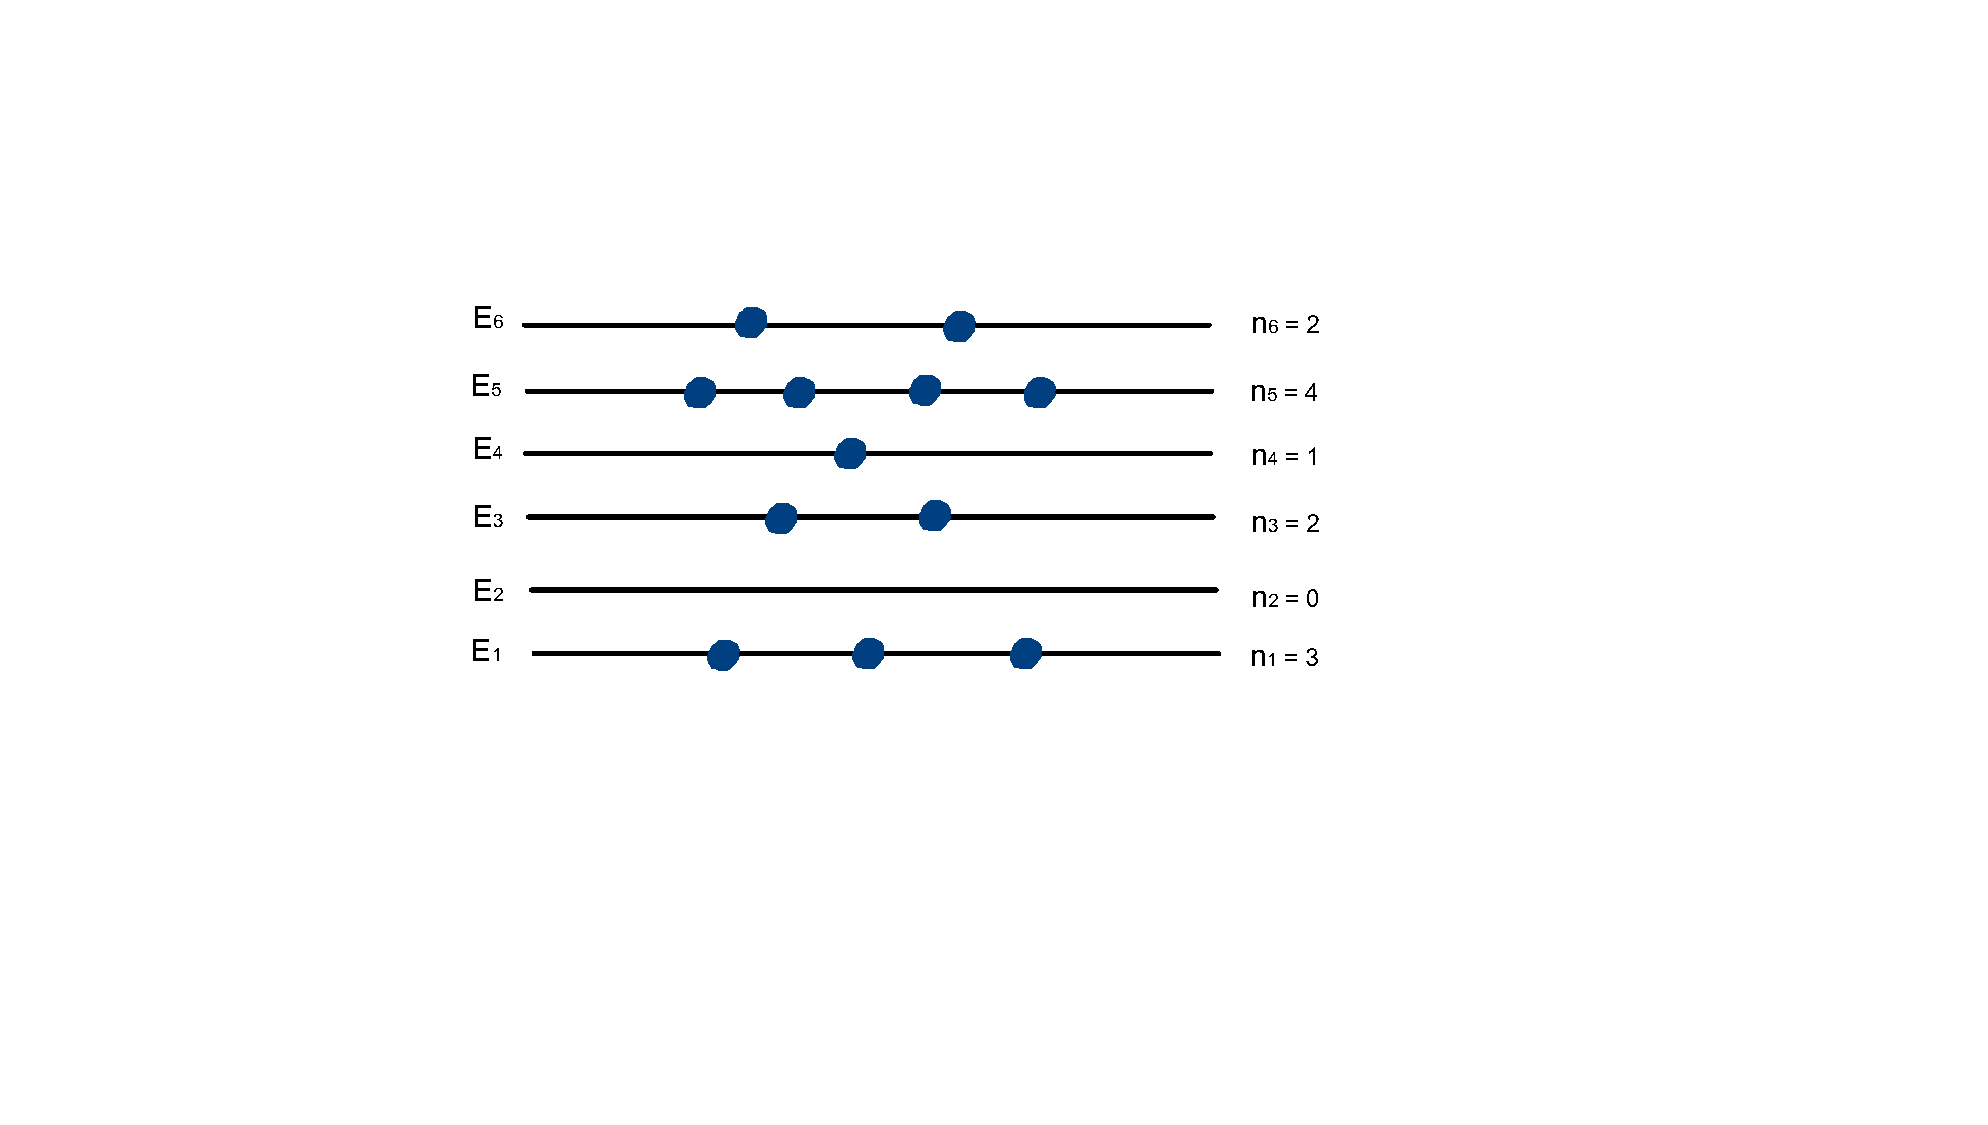
\includegraphics[scale=0.4]{/livelli_distr_particelle}
\caption{Esempio rappresentativo di una partizione, per la distribuzione di Maxwell-Boltzmann}
\label{esempio_partizione}
\end{figure}
Assumiamo che ognuno di questi livelli abbia la stessa probabilità di essere occupato.
La probabilità di una partizione è proporzionale al numero di modi differenti con cui le particelle possono essere distribuite tra i livelli di energia per produrre la partizione stessa.

Analizziamo ad esempio il caso in figura \ref{esempio_partizione}, vogliamo contare il numero di modi diversi con cui ottenere tale partizione.
Suppongo di avere un sistema a $N$ particelle.
Il modo di "piazzare" le prime tre particelle è dato dal prodotto
\begin{equation}
N (N-1) (N-2) = \frac{N!}{(N-3)!}
\end{equation}
\begin{figure}[h]
\centering
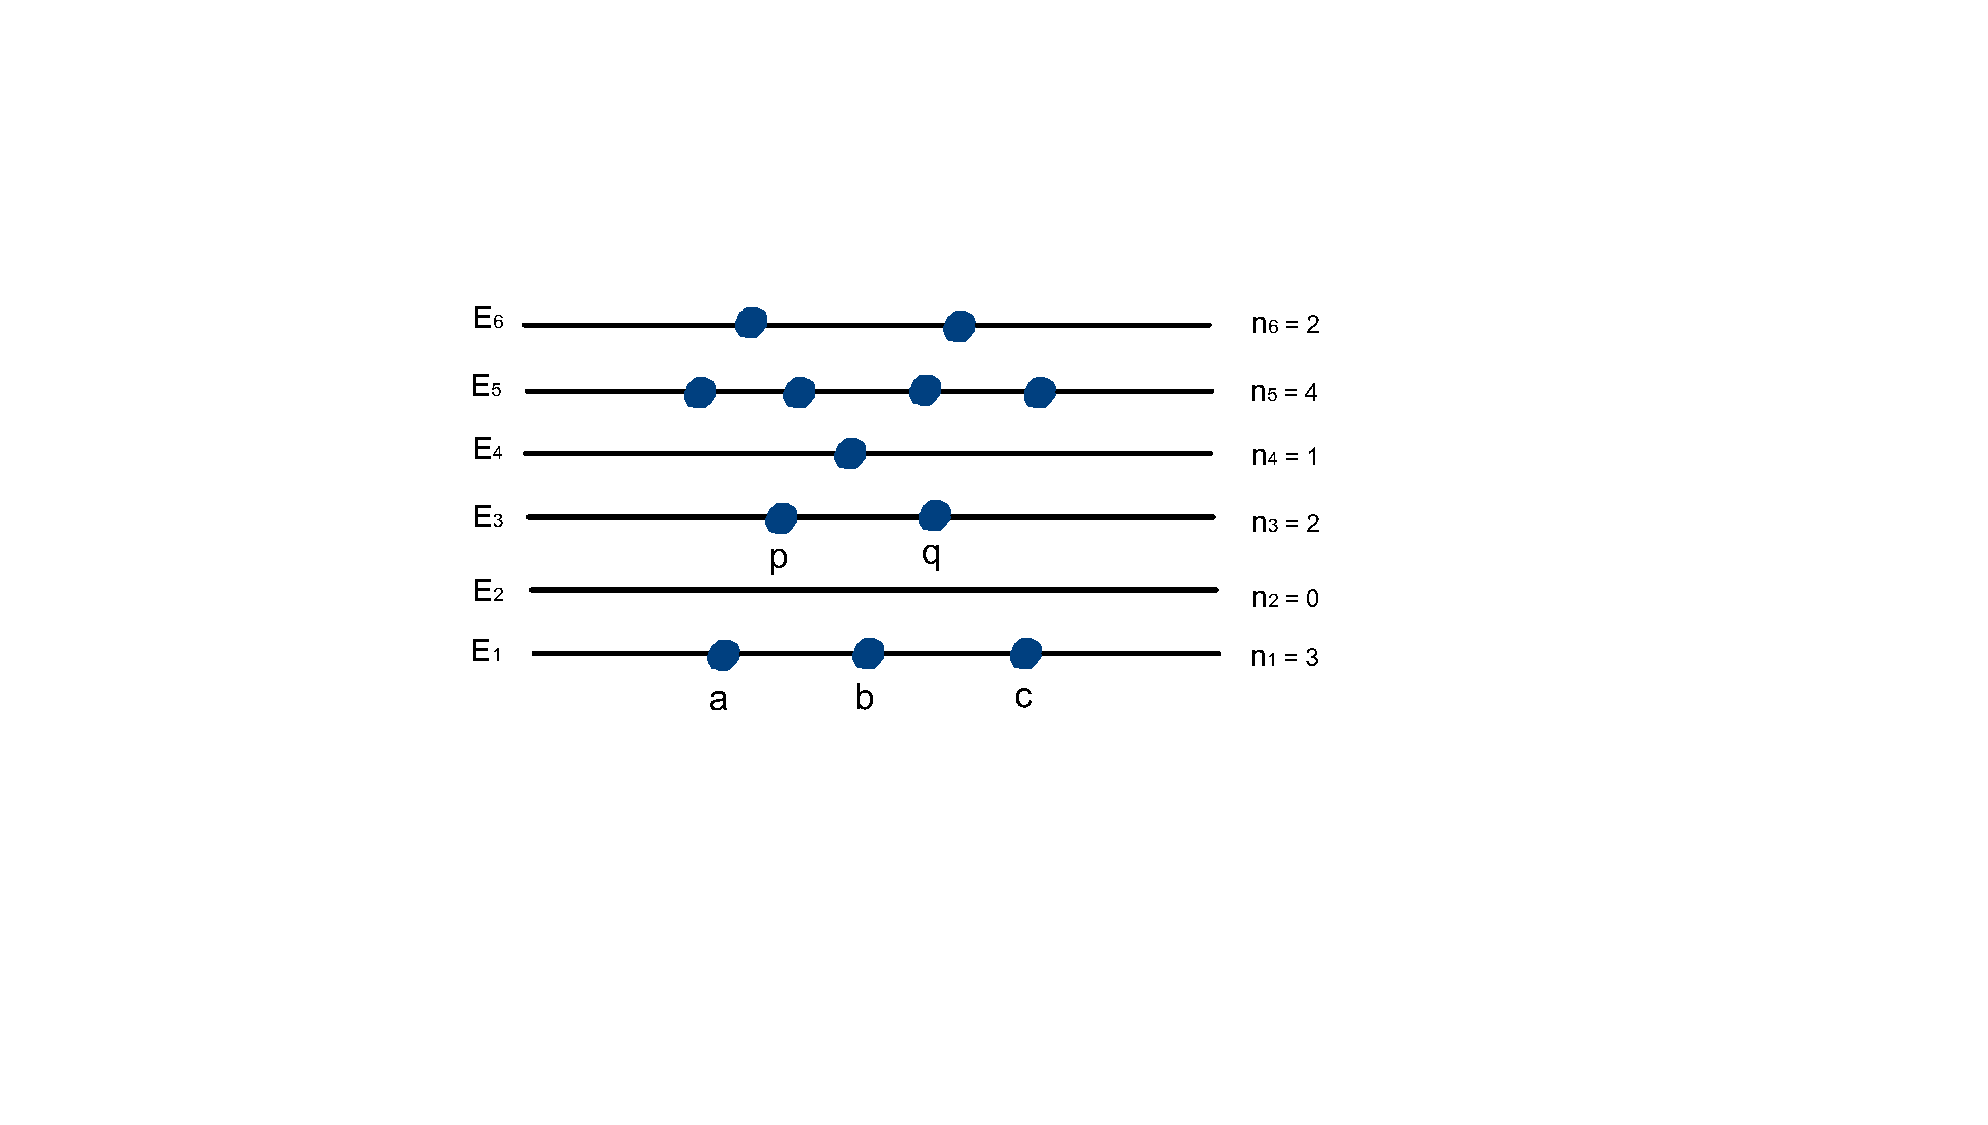
\includegraphics[scale=0.4]{/particelle_abc}
\caption{Esempio rappresentativo di una partizione, per la distribuzione di Maxwell-Boltzmann}
\label{esempio_partizione}
\end{figure}
Se le particelle fossero $a,b,c$, potrei sceglierle in 6 diversi ordini dati da
\begin{equation}
\begin{split}
& 3! = 6 \mbox{ diversi ordini} \\
& abc, bca, cab, bac, acb, cba
\end{split}
\end{equation}
questi 6 diversi ordini corrispondono alla stessa partizione, allora il numero precedente lo devo dividere per un fattore $3!$ ovvero
\begin{equation}
N (N-1) (N-2) = \frac{N!}{3!(N-3)!}
\end{equation}
Per cui generalizzando il problema: il numero di modi distinti $P_1$ di mettere $n_1$ particelle nel livello $E_1$ è
\begin{equation}
P_1 = \frac{ N!}{n_1! (N-n_1)! }
\label{stat_class}
\end{equation}
Considerando il secondo livello: ho a disposizione un numero $N-n_1$ particelle, per cui il numero di modi distinti $P_2$ di mettere $n_2$ particelle nel livello $E_2$ sarà dato da
\begin{equation}
P_2 = \frac{ (N-n_1)!}{n_2! (N-n_1-n_2)! }
\end{equation}
Analogamente per il terzo stato
\begin{equation}
P_3 = \frac{(N-n_1 - n_2)!}{n_3! ( N - n_1 - n_2 - n_3)!}
\end{equation}
Estendendo questo ragionamento si trova il seguente risultato per il livello $P_s$
\begin{equation}
P_s = \frac{(N-n_1 - n_2 - ... - n_{s-1})!}{n_s! ( N - n_1 - n_2 - ... - n_{s})!}
\end{equation}
da cui si ricava $W$, che indica il numero di modi diversi totali per fare la partizione, nel quale molti termini si semplificano:
\begin{equation}
W =  \frac{N!}{n_1! n_2! n_3! ... } = \prod_s P_s
\end{equation}
La probabilità di trovare la partizione è proporzionale al numero $W$: più tale numero è alto, più è alta la probabilità che quella partizione si realizzi.

\paragraph{Livelli degeneri}
È necessario tener conto della correzione dovuta alla \textit{degenerazione}: più stati (diversi) corrispondono alla stessa energia, per cui ad esempio potrò distribuire le $n_1$ particelle che stanno nel livello $E_1$ in $g_1^{n_1}$ (inteso come $g_1$ elevato alla $n_1$) modi diversi.
Rispetto a quanto ricavato sopra, per il livello 1 il risultato si modifica con l'aggiunta del fattore motiplicativo $g_1^{n_1}$
\begin{figure}[h]
\centering
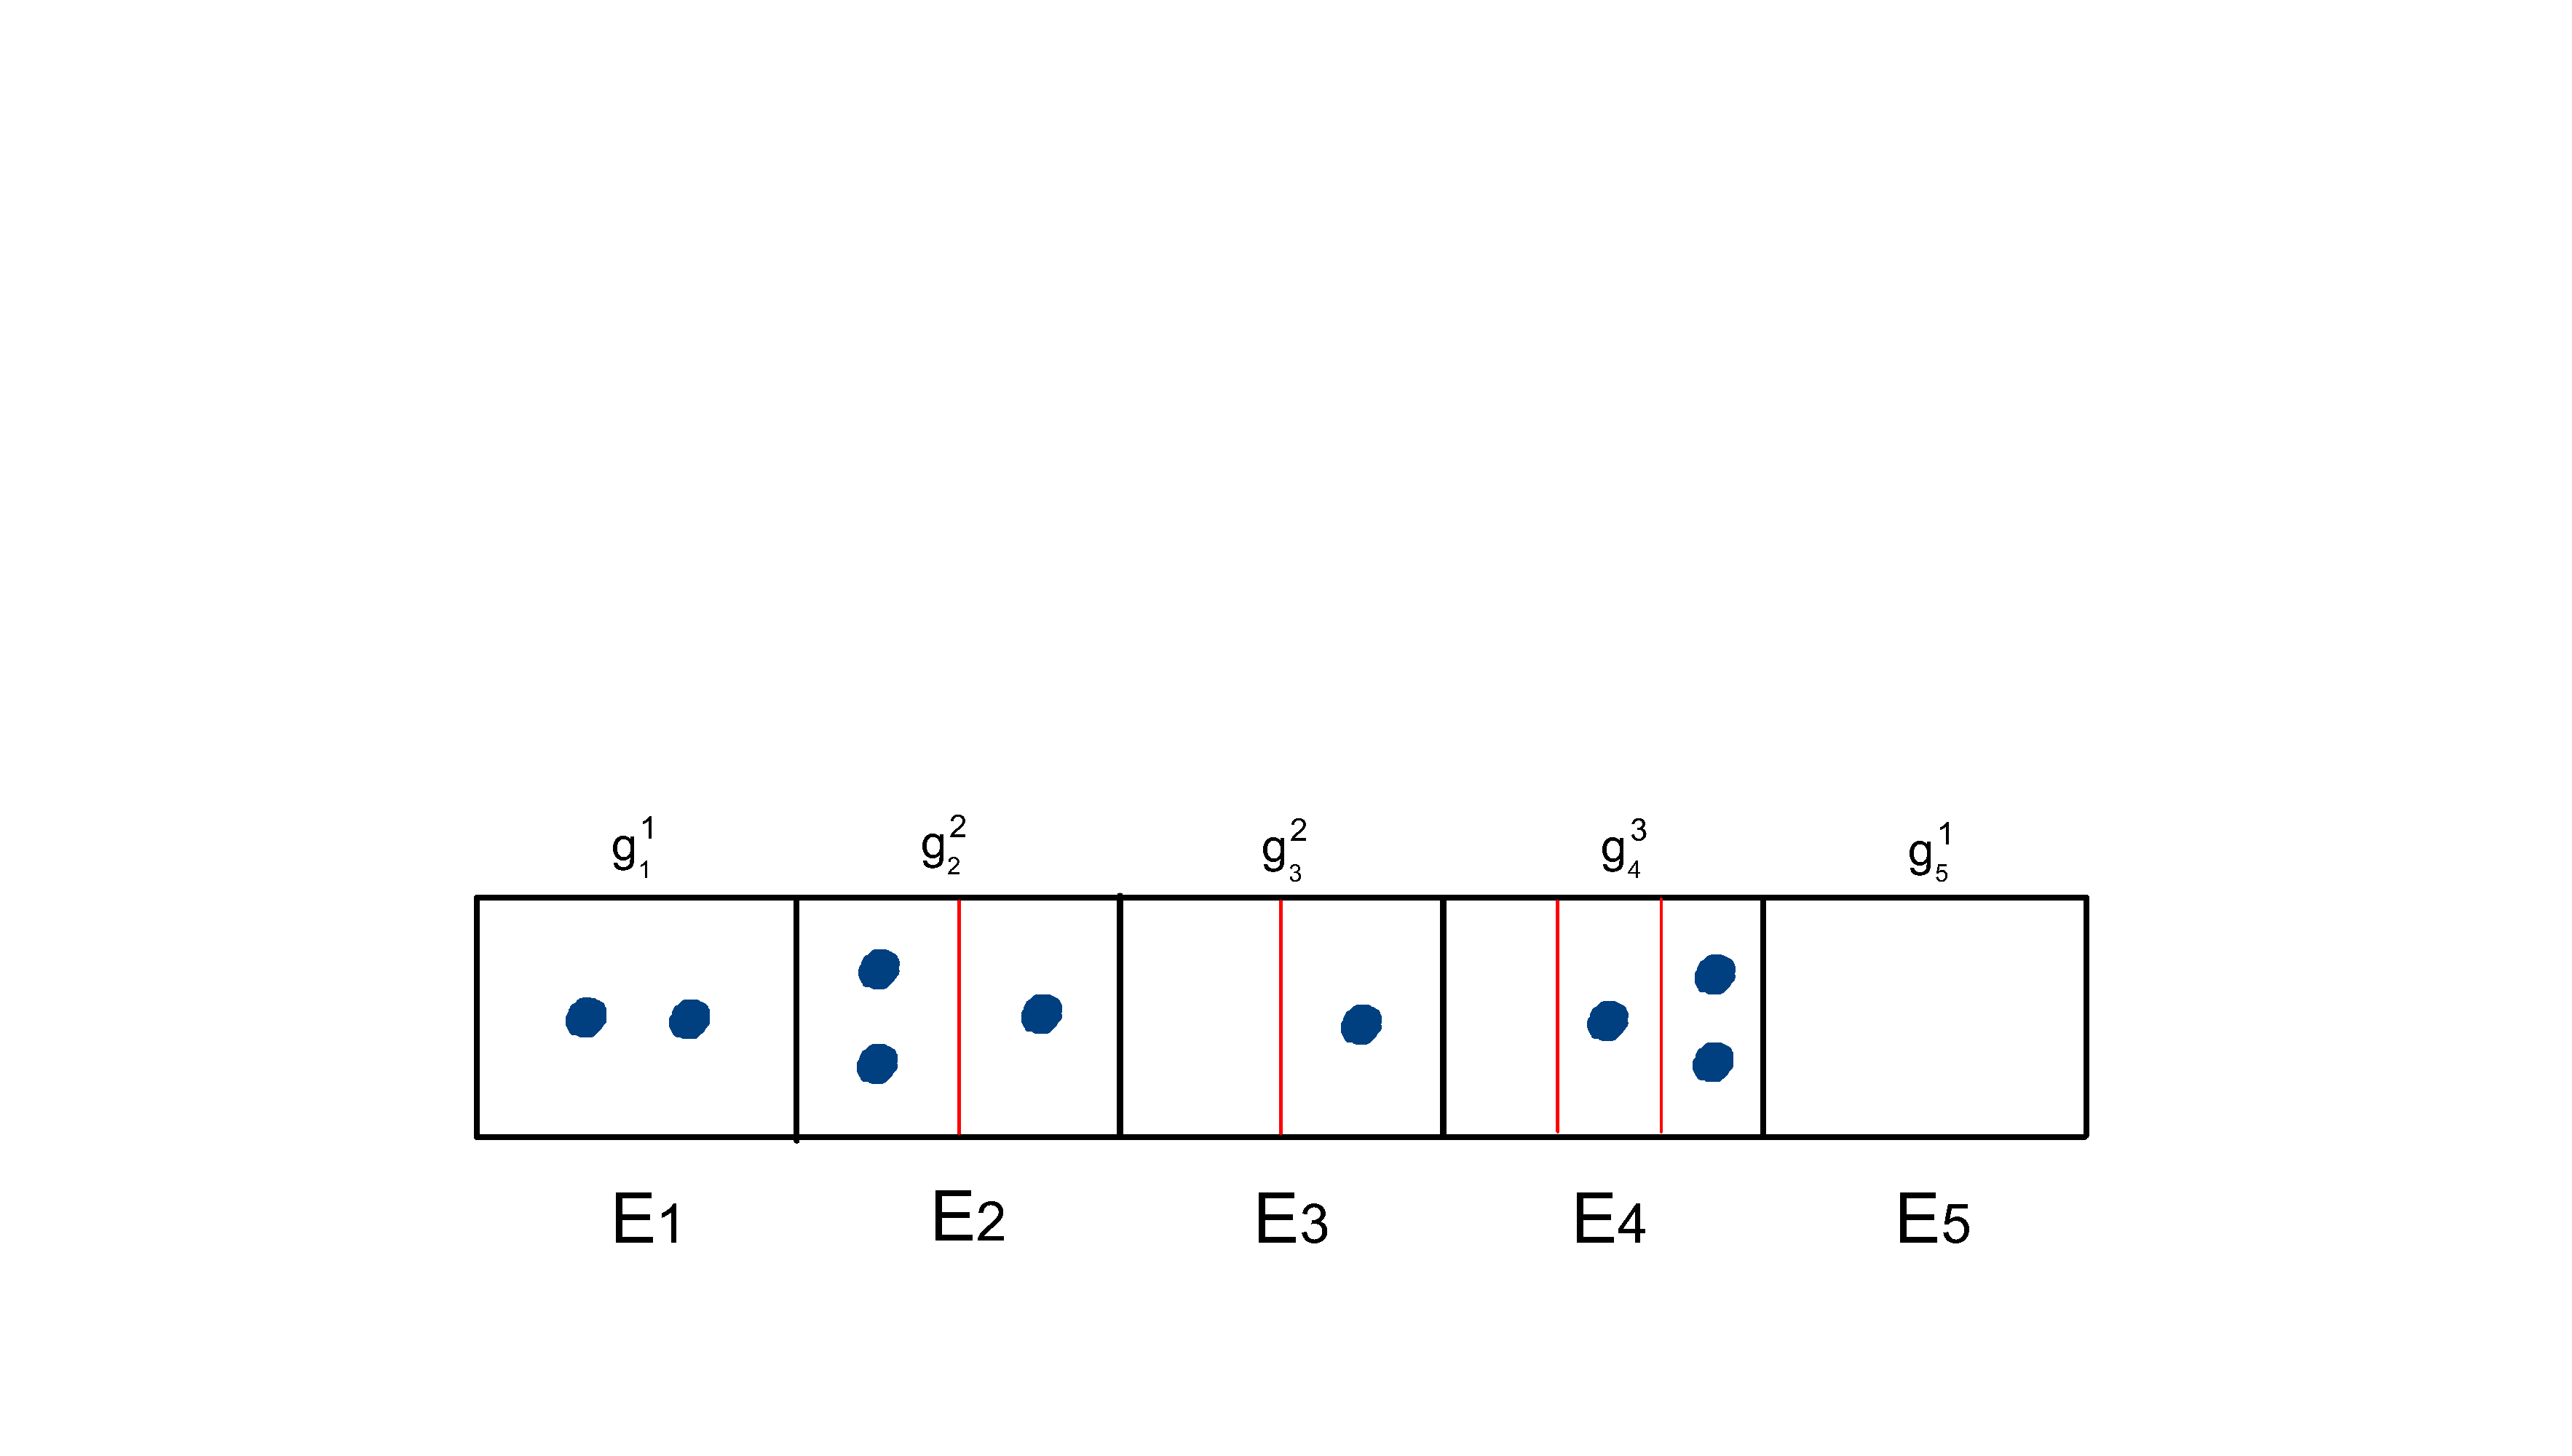
\includegraphics[scale=0.25]{/livelli_degeneri}
\caption{Livelli degeneri}
\label{esempio_partizione}
\end{figure}
\begin{equation}
P_1 = \frac{ N! g_1^{n_1}}{n_1! (N-n_1)! }
\end{equation}
analogo per tutti gli stati, quindi per lo stato $P_s$ ho
\begin{equation}
P_s = \frac{g_s^{n_s}(N-n_1 - n_2 - ... - n_{s-1})!}{n_s! ( N - n_1 - n_2 - ... - n_{s})!}
= \frac{g_s^{n_s}(N- \sum_{i=1}^{s-1}n_i )!}{n_s! ( N - \sum_{i=1}^{s}n_i )!}
\end{equation}
Il numero di modi totali distinti $W$ sarà quindi dato da
\begin{equation}
W(n_1,...,n_s) = \prod_{s=1}^{\infty} P_s = N! \prod_{s=1}^{\infty}\frac{ g_s^{n_s}}{ n_s!}
\end{equation}

\paragraph{La distribuzione più probabile è quella che massimizza il numero $W$} è il concetto chiave della meccanica statistica.
Vediamo ora come ricavare il set di numeri $n_1 ... n_s$ che massimizza $W$, tenendo presente le due condizioni iniziali: 
\begin{equation}
N  =  \sum_{s=1}^{\infty} n_s 
\quad\quad\quad
U =  \sum_{s=1}^{\infty} n_s E_s
\end{equation}
il numero delle particelle iniziali $N$ è fisso e l'energia totale è costante $U$.

Se invece di massimizzare $W$ si massimizza $\ln(W)$, i prodotti diventano somme che mi agevolano i conti, questa operazione è consentita poiché valida in generale tra $f(x)$ e $\ln(f(x))$.
Quindi significa
\begin{equation}
\delta ( W) = 0 \quad \Leftrightarrow  \quad \delta (\ln W) = 0
\end{equation}

\begin{equation}
\delta (\ln W) = \frac{ \partial (\ln W)}{\partial n_s } \delta n_s = 0
\label{massimizzare}
\end{equation}
$\delta n_s$ rappresenta la \textit{piccola variazione} sul numero $n_s$, che dovrà essere anch'essa compatibile con i due vincoli
\begin{equation}
\delta N = \sum_{s=1}^{\infty} \delta n_s = 0
\quad\quad\quad
\delta U = \sum_{s=1}^{\infty} E_s \delta n_s = 0
\label{vincoli}
\end{equation}
questo problema si risolve con il metodo dei \textit{moltiplicatori di Lagrange}, accorpando le equazioni \ref{massimizzare} e \ref{vincoli}
\begin{equation}
\begin{split}
& \delta (\ln W)   - \alpha \delta N  - \beta \delta U  = 0 \\
& \delta (\ln W)   - \alpha  \sum_{s=1}^{\infty} \delta n_s   - \beta  \sum_{s=1}^{\infty} E_s \delta n_s  = 0
\label{molti_lag}
\end{split}
\end{equation}
dove $\alpha$ e $\beta$ sono i coefficienti dei moltiplicatori di Lagrange, tali che $\alpha$ è il moltiplicatore collegato al vincolo riguardante il numero $N$ di particelle totali che è costante (prima equazione della \ref{vincoli}) e $\beta$ è il moltiplicatore collegato al vincolo riguardante l'energia $U$ del sistema costante (seconda equazione della \ref{vincoli}).
Analizziamo allora il logaritmo di $W$
\begin{equation}
\begin{split}
\ln W & = \ln \Bigl[ N! \prod_{s=1}^{\infty}\frac{ g_s^{n_s}}{ n_s!} \Bigr] \\
& = \ln N! + \sum_{s=1}^{\infty}\ln \frac{ g_s^{n_s}}{ n_s!}  \\
& = \ln N! + \sum_{s=1}^{\infty} (n_s \ln g_s - \ln n_s !)
\label{eq_max}
\end{split}
\end{equation}
e applichiamo l'\textit{approssimazione di Stirling} \ref{stirling} all'ultimo termine
\begin{equation}
\ln x! \to x \ln x - x \quad\quad \mbox{per } x \to \infty
\label{stirling}
\end{equation}
quindi l'equazione \ref{eq_max} diventa
\begin{equation}
\begin{split}
\ln W & = \ln N! + \sum_{s=1}^{\infty} (n_s \ln g_s - n_s \ln n_s + n_s) \\
& = \ln N! + \sum_{s=1}^{\infty} (\ln g_s - \ln n_s + 1) n_s
\end{split}
\end{equation}
Ora usando la condizione \ref{massimizzare}, eseguiamo la derivata parziale in $n_s$ e otteniamo
\begin{equation}
\begin{split}
\delta (\ln W) & = \frac{ \partial}{\partial n_s } \Bigl[ \ln N! + \sum_{s=1}^{\infty} (\ln g_s - \ln n_s + 1) n_s \Bigr]  \delta n_s \\
& = \sum_{s=1}^{\infty} (\ln g_s - \ln n_s - 1 + 1) \delta n_s \\
& = \sum_{s=1}^{\infty} (\ln g_s - \ln n_s ) \delta n_s
\end{split}
\end{equation}
sostituiamo questo risultato nell'equazione \ref{molti_lag} e otteniamo
\begin{equation}
\sum_{s=1}^{\infty} (\ln g_s - \ln n_s - \alpha - \beta E_s) \delta n_s = 0 
\end{equation}
che sarà verificata per
\begin{equation}
\begin{split}
\sum_{s=1}^{\infty} \Bigl[ \ln g_s - \ln n_s  \Bigr]\delta n_s & = \sum_{s=1}^{\infty} ( \alpha + \beta E_s) \delta n_s \\
\ln \frac{ g_s}{n_s } & = \alpha + \beta E_s \\
\frac{ g_s}{n_s } & = e^{ \alpha + \beta E_s } 
\end{split}
\end{equation}
da cui otteniamo i valori di $n_s$ in funzione di $\alpha$ e $\beta$
\begin{equation}
\frac{ n_s}{g_s } = \frac{ 1}{ e^{ \alpha + \beta E_s }  }
\label{dist_MB}
\end{equation}
arrivando infine alla \textit{Legge di distribuzione di Maxwell Boltzmann}.
Da cui possiamo ricavare la \textit{Funzione di Partizione} $Z$
\begin{equation}
\begin{split}
N & = \sum_{s=1}^{\infty} n_s = \sum_{s=1}^{\infty} g_s e^{ -\alpha } e^{ -\beta E_s } \\
e^{ -\alpha } & = \frac{ N}{ g_s  e^{ -\beta E_s }} = \frac{ N}{Z } \quad\Rightarrow\quad  Z =  \sum_{s=1}^{\infty} g_s e^{ -\beta E_s }
\end{split}
\end{equation}
e possiamo riscrivere la \textit{Legge di distribuzione di Maxwell Boltzmann} come
\begin{equation}
n_s = \frac{ N}{Z } g_s e^{ -\beta E_s }
\end{equation}
che è un'espressione dei numeri $n_s$ che massimizza il valore del numero $W$, ovvero la partizione più probabile.
Nella statistica classica di Maxwell Boltzmann $\frac{ n_s}{N }$ è la probabilità che una particella abbia energia $E_s$ e vale
\begin{equation}
\frac{ n_s }{N } = \frac{ 1}{Z } g_s e^{ -\beta E_s }
\end{equation}
che sarà anche la probabilità di occupazione del livello $E_s$.


\subsection{Statistica quantistica di Bose Einstein}
La Statistica quantistica di Bose Einstein si applica a particelle che non rispettano il Principio di esclusione di Pauli, quindi i bosoni.
Essendo particelle quantistiche e quindi non distinguibili non posso applicare la statistica classica \ref{stat_class}, ovvero non posso più contare le scelte possibili per una data particella ma considero il set di particelle tutto insieme e quello che devo considerare sono gli stati $g_s$ in un certo livello generico $E_s$ e contare il numero di modi in cui $n_s$ particelle possono andare nei $g_s$ stati del livello energetico $E_s$.
Supponiamo, ad esempio illustrativo, una schematizzazione di un unico generico livello $E_s$ come in figura \ref{livello_Es},
\begin{figure}[h]
\centering
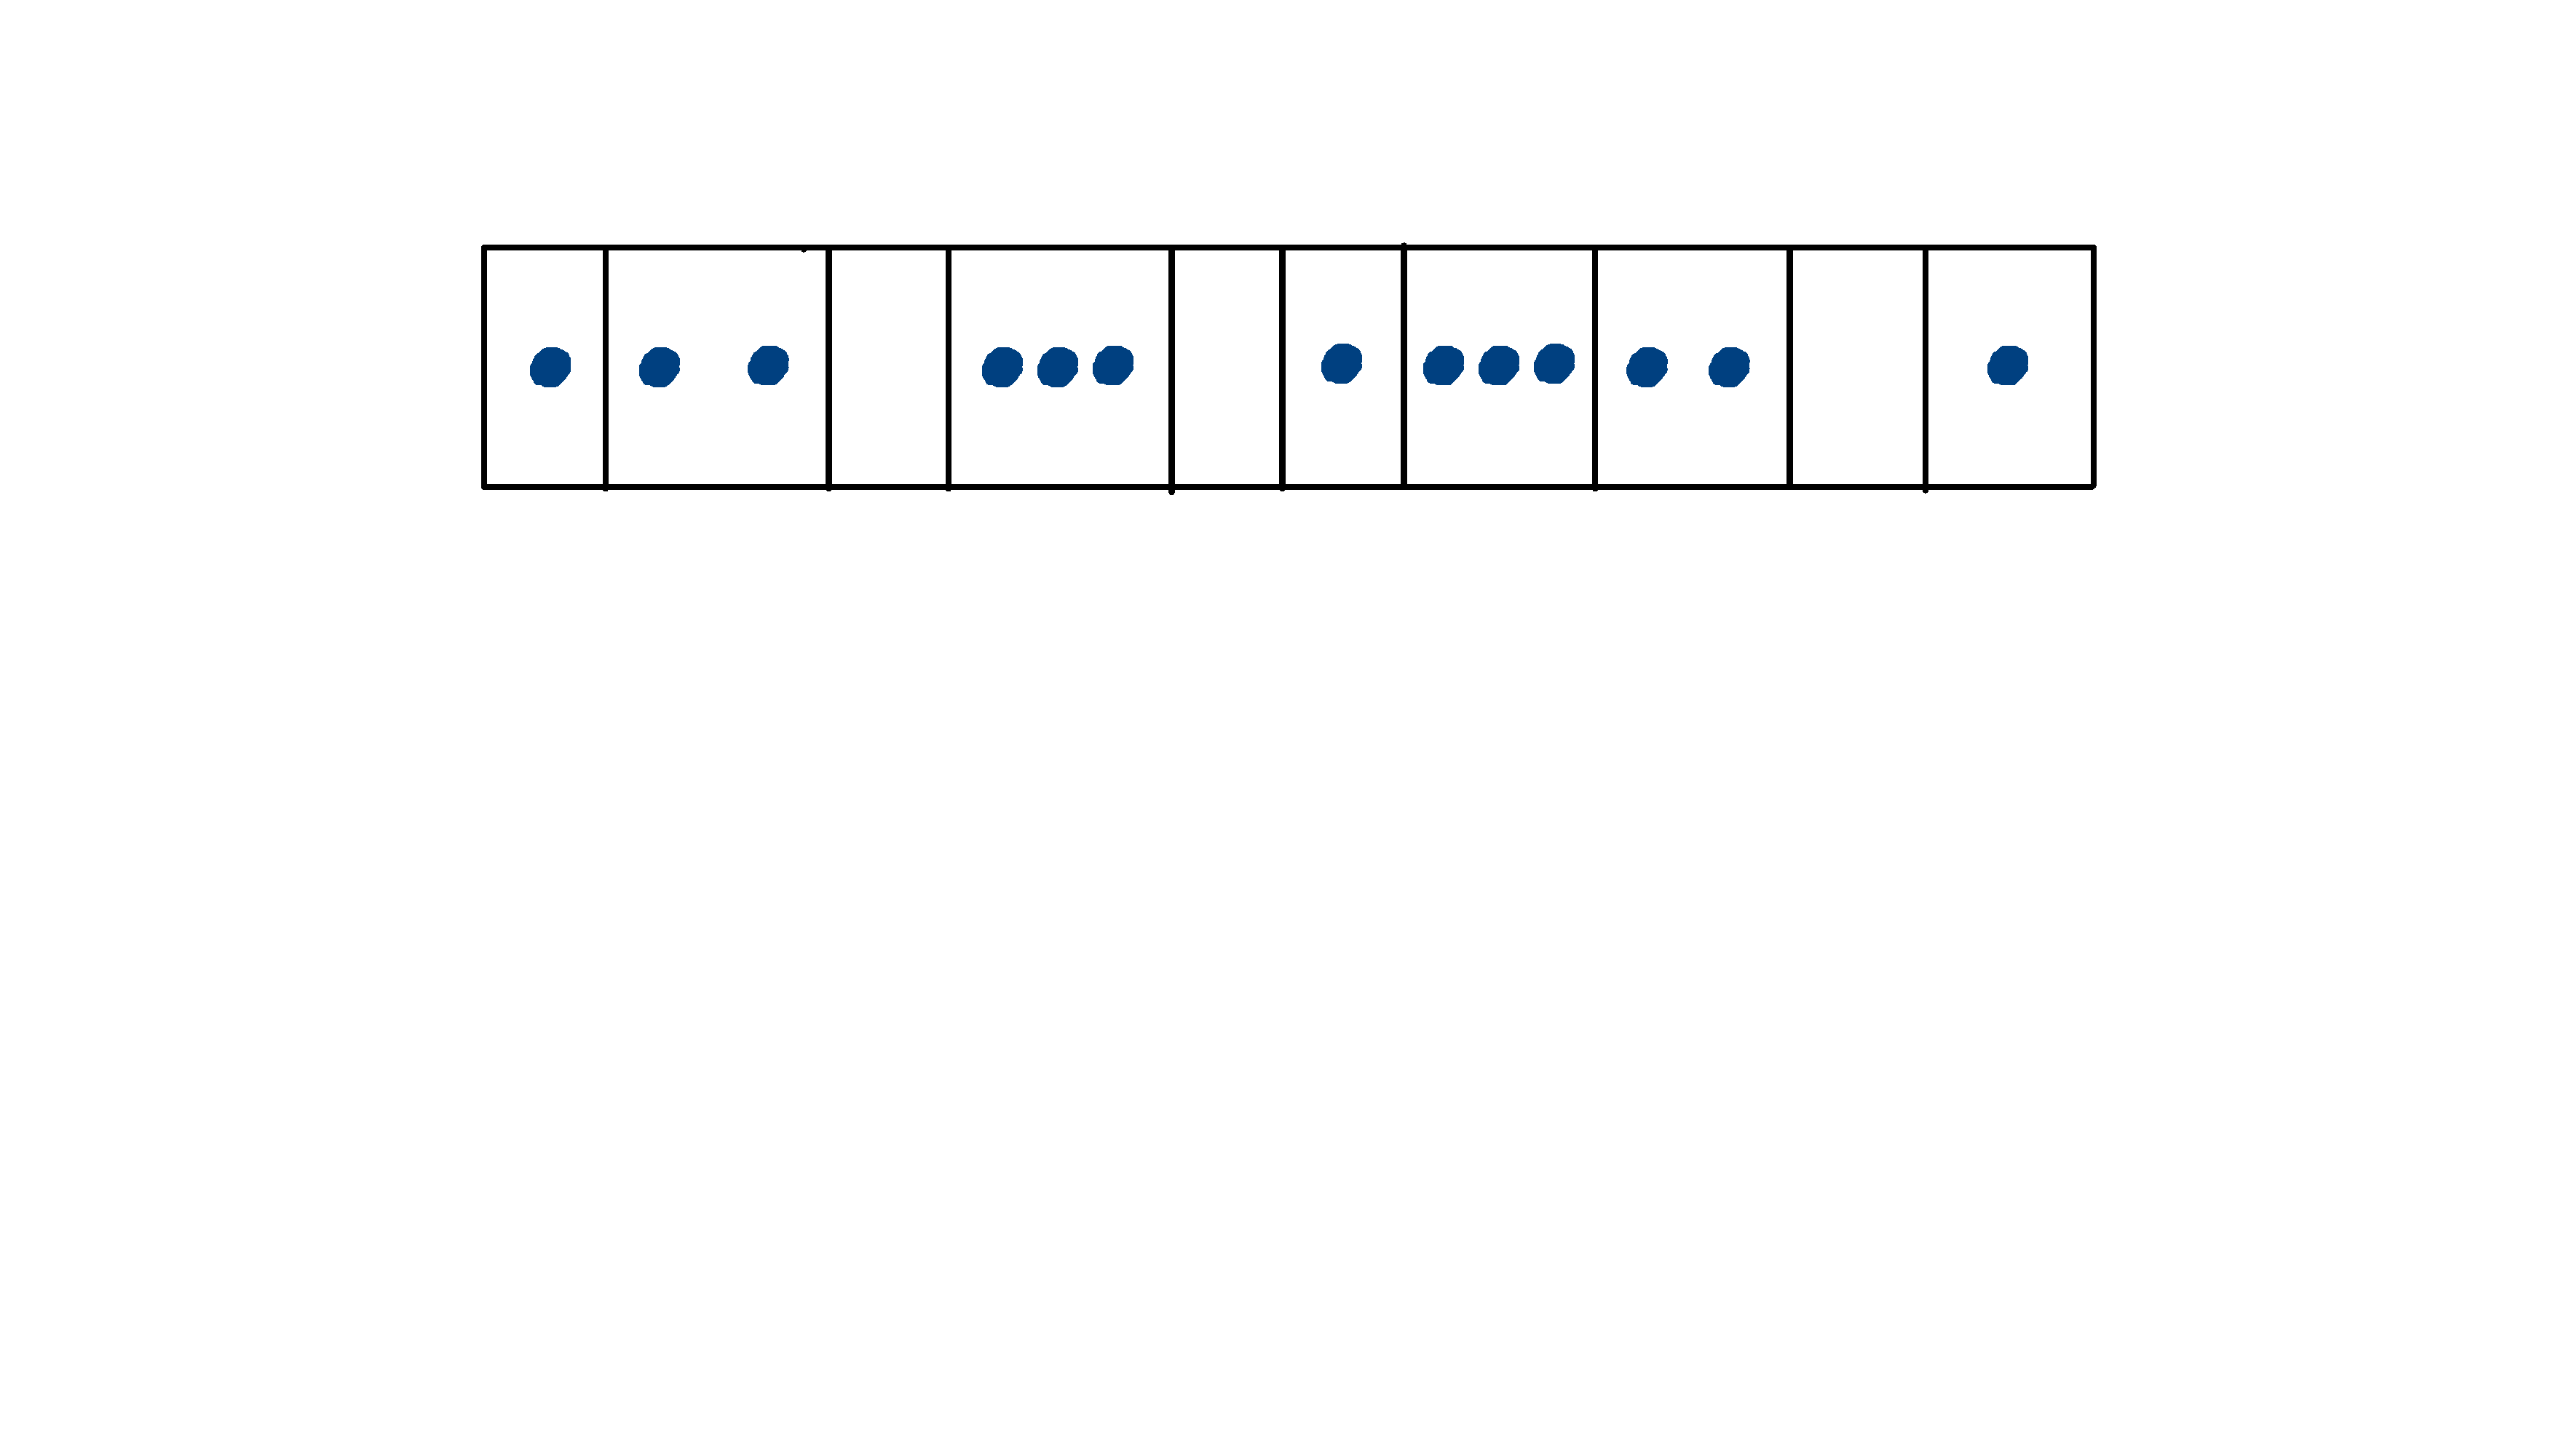
\includegraphics[scale=0.3]{/livello_Es_1}
\caption{Livello energetico $E_s$, $n_s = 13$ particelle, $g_s = 10$ stati nel livello}
\label{livello_Es}
\end{figure}
otteniamo un diverso \textit{modo} cambiando il numero di particelle in uno o più stati, ma non otteniamo un \textit{modo} nuovo se scambiamo due particelle fra loro all'interno dello stesso stato o tra i diversi stati dello stesso livello.

Per contare il numero di modi vediamo il seguente ragionamento:
ci sono $g_s - 1$ linee di divisione tra gli stati
e ci sono $n_s + g_s - 1$ particelle + linee di divisione 
quindi nel caso in esempio ho:
\begin{itemize}
\item $g_s - 1 = 10 - 1 = 9 $ \textit{linee di divisione}
\item $n_s + g_s - 1 = 13 + 10 - 1 = 22$ \textit{particelle + linee di divisione}
\end{itemize}
Posso ottenere il seguente altro \textit{modo} di figura \ref{livello_Es_2} variando la composizione dei soli primi due stati 
\begin{figure}[h]
\centering
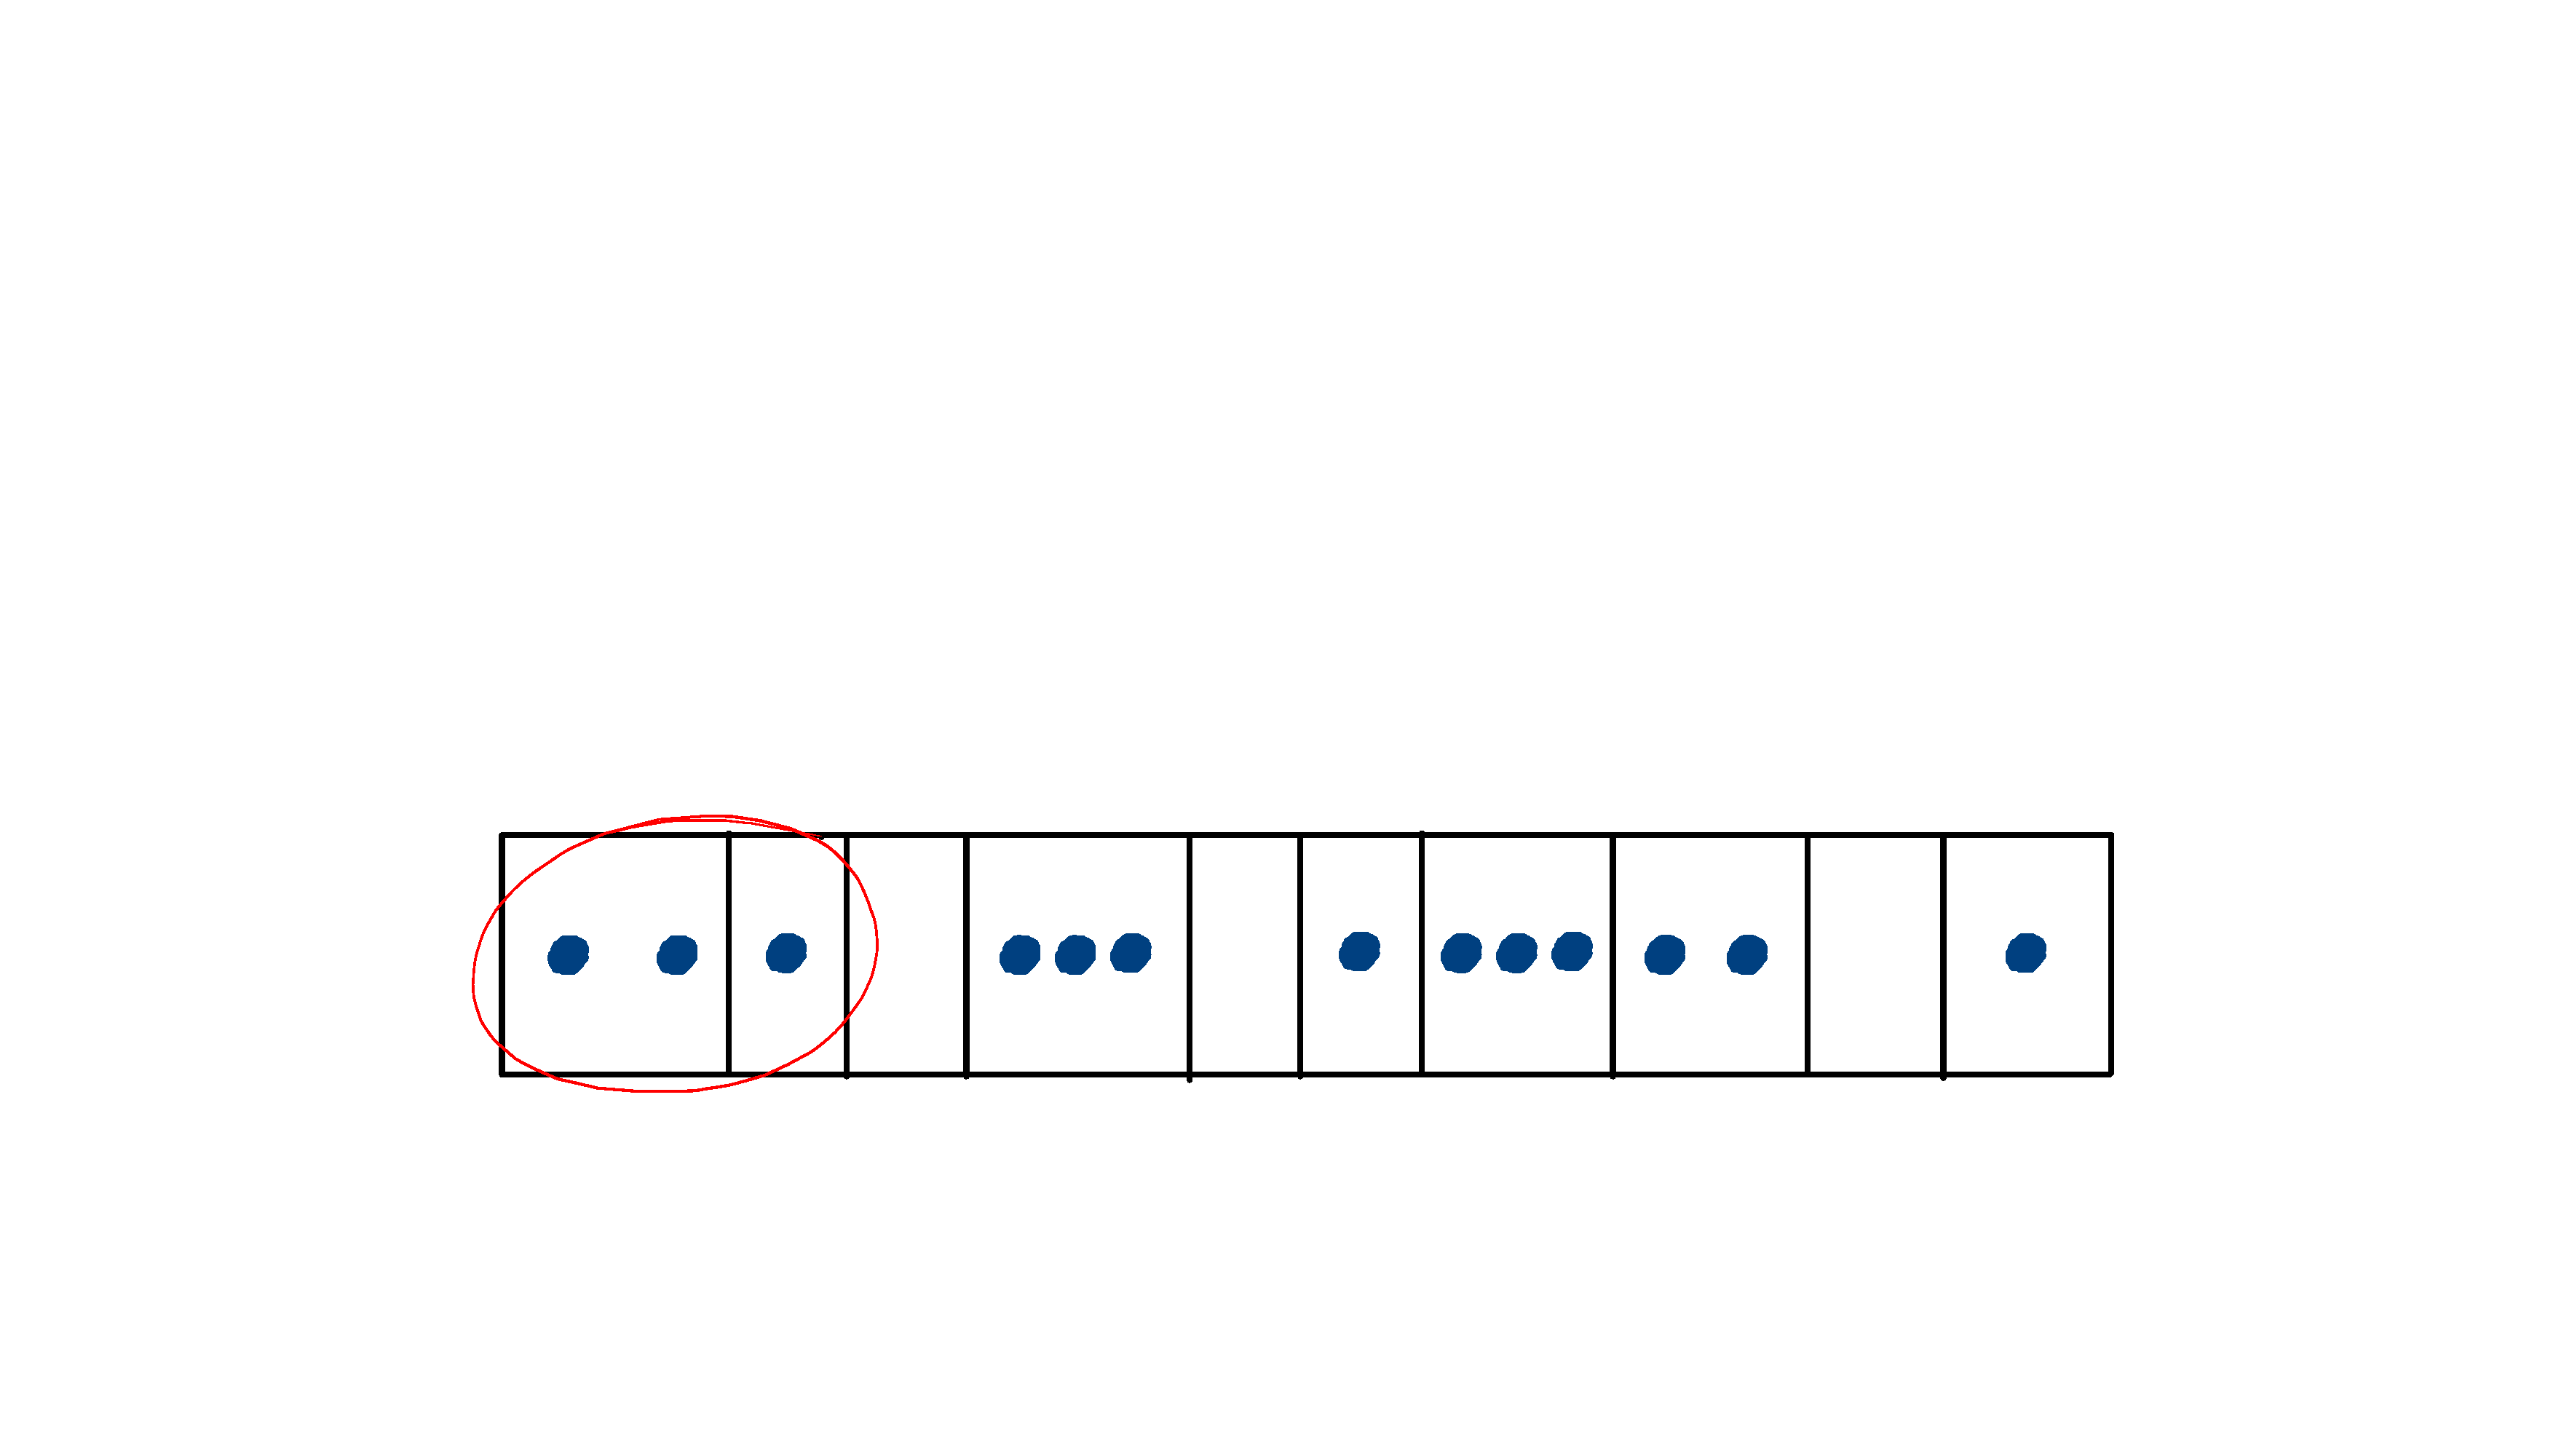
\includegraphics[scale=0.3]{/livello_Es_2}
\caption{Livello energetico $E_s$, $n_s = 13$ particelle, $g_s = 10$ stati nel livello}
\label{livello_Es_2}
\end{figure}
posso ottenerlo sia spostando una particella da uno stato all'altro sia spostando la linea di divisione e dividendo diversamente le particelle.
Quindi ci sono $(n_s + g_s - 1)!$ possibili permutazioni di particelle e linee di divisione che posso compiere, però alcune permutazioni non producono nuovi modi, quindi il numero totale di modi distinguibili di distribuire $n_s$ particelle nei $g_s$ stati del livello $E_s$ è
\begin{equation}
P_s = \frac{ (n_s + g_s - 1)!}{n_s! (g_s - 1)! }
\end{equation}
per cui il numero di modi totali è
\begin{equation}
\begin{split}
W(n_1, ..., n_s) = \prod_{s=1}^{ \infty } P_s = \prod_{s=1}^{ \infty } \frac{ (n_s + g_s - 1)!}{n_s! (g_s - 1)! }
\end{split}
\end{equation}
Quindi ora, come visto nella statistica precedente, cerco di massimizzare il numero $W$, ovvero massimizzo $\ln W$, utilizzando l'approssimazione di Stirling, in cui approssimo per $(x+1) \to x$ quando $x \to \infty$
\begin{equation}
\ln (x+1)! \to x \ln x - x \quad\quad \mbox{per } x \to \infty
\label{stirling_2}
\end{equation}
e trovo
\begin{equation}
\begin{split}
\ln W & = \sum_{s=1}^{\infty} \Bigl[ \ln ( n_s + g_s - 1 )! - \ln n_s ! - \ln (g_s - 1)! \Bigr] \\
& = \sum_{s=1}^{\infty} \Bigl[ ( n_s + g_s )(\ln ( n_s + g_s ) - 1) - n_s (\ln n_s -1 ) - g_s (\ln g_s - 1) \Bigr]
\end{split}
\end{equation}
che differenziata diventa
\begin{equation}
\delta (\ln W) = \sum_{s=1}^{\infty} \Bigl[ \ln(n_s + g_s) - \ln n_s \Bigr] \delta n_s
\end{equation}
inserendo questo risultato nella \ref{molti_lag} ottengo l'equazione 
da cui posso ottenere i valori di $n_s$ in funzione di $\alpha$ e di $\beta$
\begin{equation}
\sum_{s=1}^{\infty} \Bigl[ \ln(n_s + g_s) - \ln n_s - \alpha -\beta E_s\Bigr] \delta n_s = 0
\end{equation}
verificata per 
\begin{equation}
\begin{split}
\sum_{s=1}^{\infty} \Bigl[ \ln \Bigl(  1 + \frac{ g_s}{n_s }  \Bigr) \Bigr]\delta n_s & = \sum_{s=1}^{\infty} \Bigl[ \alpha + \beta E_s \Bigr]\delta n_s \\
\ln \Bigl(  1 + \frac{ g_s}{n_s}  \Bigr) &= \alpha + \beta E_s \\
1 + \frac{ g_s}{n_s} & = e^{ \alpha + \beta E_s  }
\end{split}
\end{equation}
arrivando infine alla \textit{Legge di distribuzione di Bose Einstein}
\begin{equation}
\frac{ n_s}{g_s } = \frac{ 1}{e^{\alpha +\beta E_s} - 1 }
\label{dist_BE}
\end{equation}



\subsection{Statistica quantistica di Fermi Dirac}
La Statistica quantistica di Fermi Dirac si applica a particelle che obbediscono al Principio di esclusione di Pauli, quindi i fermioni.
Considero un livello energetico $E_s$ in cui ho $n_s$ particelle e $g_s$ stati disponibili e però devo tenere conto del principio di esclusione di Pauli, quindi devo contare i modi possibili per la partizione con la condizione che non ci sia più di una particella per ogni stato.
Possiamo allora dividere tutti gli stati in \underline{due gruppi}: $n_s$ sono tutti gli stati occupati e $(g_s - n_s)$ sono tutti gli stati non occupati.
Per cui il numero di modi è
\begin{equation}
P_s = \frac{ g_s !}{n_s! (g_s - n_s)! }
\end{equation}
che è analogo nella statistica classica per $P_1$ del primo livello...
Il numero totale $W$ è
\begin{equation}
W = \prod_{s=1}^{\infty} P_s = \prod_{s=1}^{\infty} \frac{ g_s !}{n_s! (g_s - n_s)! }
\end{equation}
quindi come nei casi precedenti
\begin{equation}
\begin{split}
\ln W & = \sum _{s=1}^{\infty} \Bigl[  \ln g_s! - \ln n_s! - \ln (g_s -n_s)!  \Bigr] \\
& = \sum _{s=1}^{\infty} \Bigl[   g_s \ln g_s - n_s \ln n_s  - (g_s - n_s) \ln (g_s - n_s)  \Bigr]
\end{split}
\end{equation}
che differenziata diventa
\begin{equation}
\delta (\ln W) = \sum _{s=1}^{\infty} \Bigl[ \ln (g_s - n_s) - \ln n_s \Bigr] \delta n_s
\end{equation}
da cui poi si applica la tecnica dei Moltiplicatori di Lagrange
\begin{equation}
\sum _{s=1}^{\infty} \Bigl[   \ln (g_s - n_s) - \ln n_s - \alpha - \beta E_s  \Bigr] \delta n_s = 0
\end{equation}
verificata per
\begin{equation}
\begin{split}
\sum _{s=1}^{\infty} \Bigl[   \ln (g_s - n_s) - \ln n_s \Bigr] \delta n_s &= \sum _{s=1}^{\infty} \Bigl[ \alpha + \beta E_s  \Bigr] \delta n_s \\
\ln \Bigl(  \frac{g_s }{n_s } - 1  \Bigr) & =  \alpha + \beta E_s \\
\frac{g_s }{n_s } - 1 & =  e^{ \alpha + \beta E_s  }
\end{split}
\end{equation}
arrivando infine alla \textit{Legge di distribuzione di Fermi Dirac}
\begin{equation}
\frac{ n_s}{g_s } = \frac{ 1}{e^{ \alpha + \beta E_s } + 1 }
\label{dist_FD}
\end{equation}


\subsection{Riassunto statistiche}
Distribuzione di Maxwell Boltzmann (eq \ref{dist_MB})
\begin{equation}
P_s = \frac{g_s^{n_s}(N- \sum_{i=1}^{s-1}n_i )!}{n_s! ( N - \sum_{i=1}^{s}n_i )!}  
\quad\quad\quad  
W = N! \prod_{s=1}^{\infty}\frac{ g_s^{n_s}}{ n_s!}
\quad\quad\quad  
\frac{ n_s}{g_s } = \frac{ 1}{e^{ \alpha + \beta E_s } }
\end{equation}
Distribuzione di Bose Einstein (eq \ref{dist_BE})
\begin{equation}
P_s = \frac{ (n_s + g_s - 1)!}{n_s! (g_s - 1)! }  
\quad\quad\quad 
W =  \prod_{s=1}^{ \infty } \frac{ (n_s + g_s - 1)!}{n_s! (g_s - 1)! }
\quad\quad\quad
\frac{ n_s}{g_s } = \frac{ 1}{e^{ \alpha + \beta E_s } - 1 }
\end{equation}
Distribuzione di Fermi Dirac (eq \ref{dist_FD})
\begin{equation}
P_s = \frac{ g_s !}{n_s! (g_s - n_s)! }
\quad\quad\quad
W = \prod_{s=1}^{\infty} \frac{ g_s !}{n_s! (g_s - n_s)! }
\quad\quad\quad
\frac{ n_s}{g_s } = \frac{ 1}{e^{ \alpha + \beta E_s } + 1 }
\end{equation}

\paragraph{plot}
Nei seguenti grafici sono riportati i plot di $\frac{ n_s}{g_s }$ in funzione di $E_s$, \\
ponendo i parametri $\alpha=\beta=1$
\begin{figure}[h]
\centering
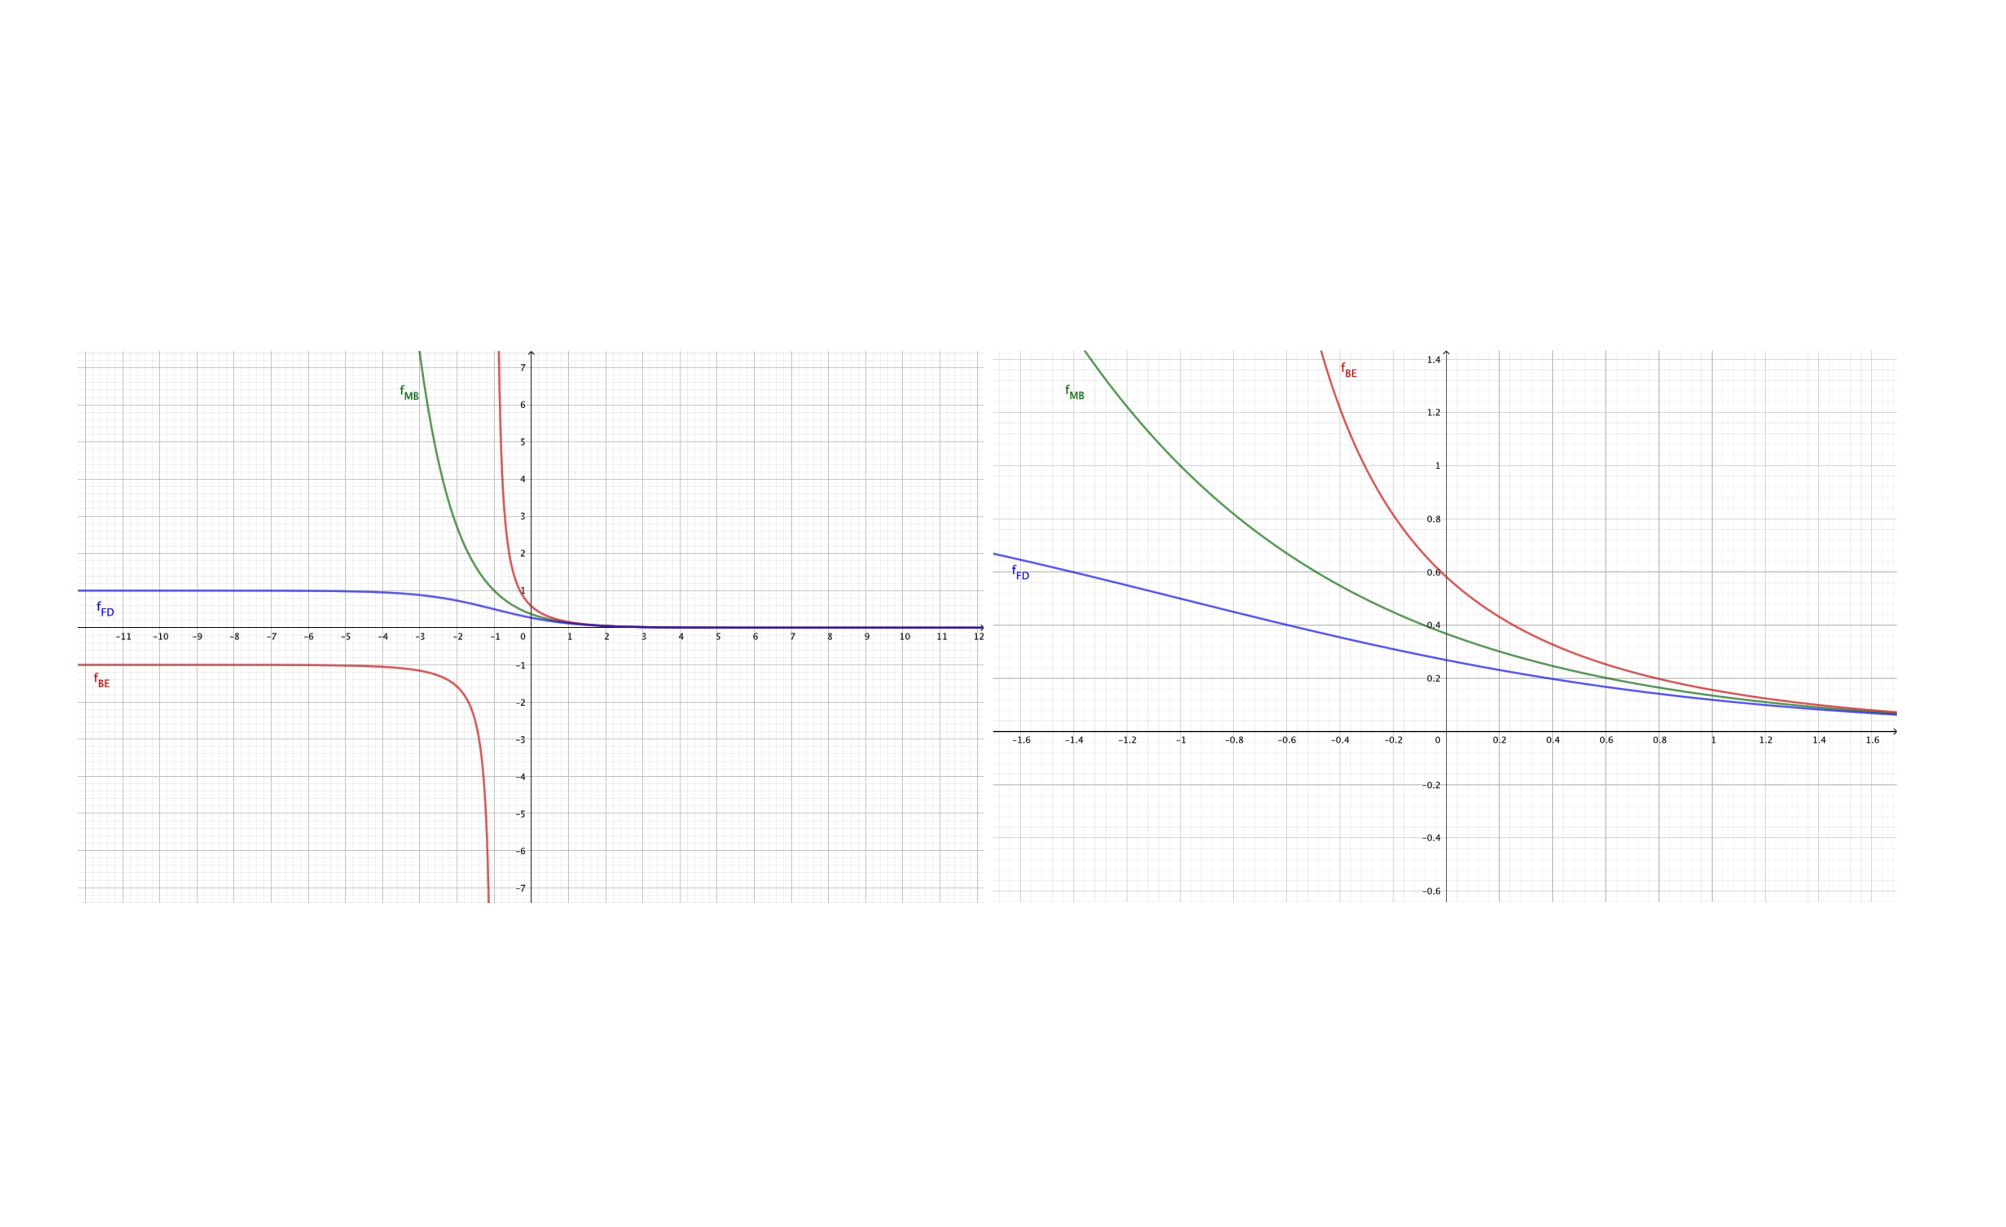
\includegraphics[scale=0.54]{/plot_distrib_oriz}
\end{figure}


